% !TEX root=../../mt-motion-analysis.tex
%!TeX spellcheck = en-US
\chapter{Methods} \label{ch:method}
\section{Overview}
In this chapter, the system for assessing POEs will be presented. This system is naturally divided into two parts where firstly the videos are analyzed. The first subsystem extracts body part coordinates of the subjects. This information is then passed to the second subsystem where it is used to calculate a score according to \cite{Nae2020b}. The data used is presented in Section \ref{sec:met-data} and the two subsystems are described in Sections \ref{sec:met-loc} and \ref{sec:met-class}, respectively.

\section{Data}\label{sec:met-data}
The data available is in the form of videos each containing one subject, recorded from a frontal view. As discussed in Chapter \ref{ch:intro}, the \gls{sls} task and the trunk, pelvis, femoral valgus, and \gls{kmfp} \glspl{poe} are evaluated. Each video contains four-five repetitions and for each repetition the \glspl{poe} above have been scored according to Table \ref{tab:poes}. Along with the \gls{poe} scores a certainty score, describing the confidence of the physiotherapist assessing the videos, is provided. This is between 0 (certain) and 2 (uncertain) and when above 0 the uncertainty direction is provided as well. This certainty score is only available for the combined (median) score for all repetitions, i.e. one certainty score per video.

In total there are labeled videos from 103 different subjects and for some of the subjects there are videos of the task performed with both right and left leg. The number of labeled repetitions per video and \gls{poe} varies slightly. This variation is due to different factors such as all subjects not performing five repetitions, or that the entire movement was not captured in the video and was thereby excluded by us. The total amount of data for the different \glspl{poe} is summarized in Table \ref{tab:data}. From this data 22 of the repetition sequences (110 repetitions), from 22 different subjects, were put aside as a test set. The test set was chosen from the set of repetition sequences ensuring no data from the same sequence was in both the training and test data.

The label distributions can be seen in Figure \ref{fig:label-dist} and it can be noted that for all \glspl{poe} there is a slight imbalance with fewer repetitions classified as Poor. The imbalance for \gls{kmfp} is very clear with about 80\% of the data classified as Good. In the same figure the label distribution  for the test set is shown as well. For the trunk \gls{poe} it is slightly different from its overall distribution while similar for the other sets.

\begin{table}
 \centering
 \caption{Data available for the different POEs.}
 \label{tab:data}
 % \footnotesize
 % {\renewcommand{\arraystretch}{1.2}
 % {\tabulinesep=0.8mm
 \begin{tabu}[t]{cccc}
   \textbf{\gls{poe}} &
   \multicolumn{1}{c}{\begin{tabular}[c]{@{}c@{}}\textbf{Number of}\\\textbf{unique subjects}\end{tabular}} &
   \multicolumn{1}{c}{\begin{tabular}[c]{@{}c@{}}\textbf{Number of}\\\textbf{repetition sequences}\end{tabular}} &
   \multicolumn{1}{c}{\begin{tabular}[c]{@{}c@{}}\textbf{Number of}\\ \textbf{repetitions}\end{tabular}} \\ \hline \hline
   \textbf{Trunk} & 103 & 105 & 520 \\
   \textbf{Pelvis} & 103 & 105 & 519 \\
   \textbf{Femoral Valgus} & 103 & 107 & 530 \\
   \textbf{\gls{kmfp}} & 103 & 107 & 530

 \end{tabu}

\end{table}

\begin{figure}
  \centering
  \begin{subfigure}[t]{0.24\textwidth}
    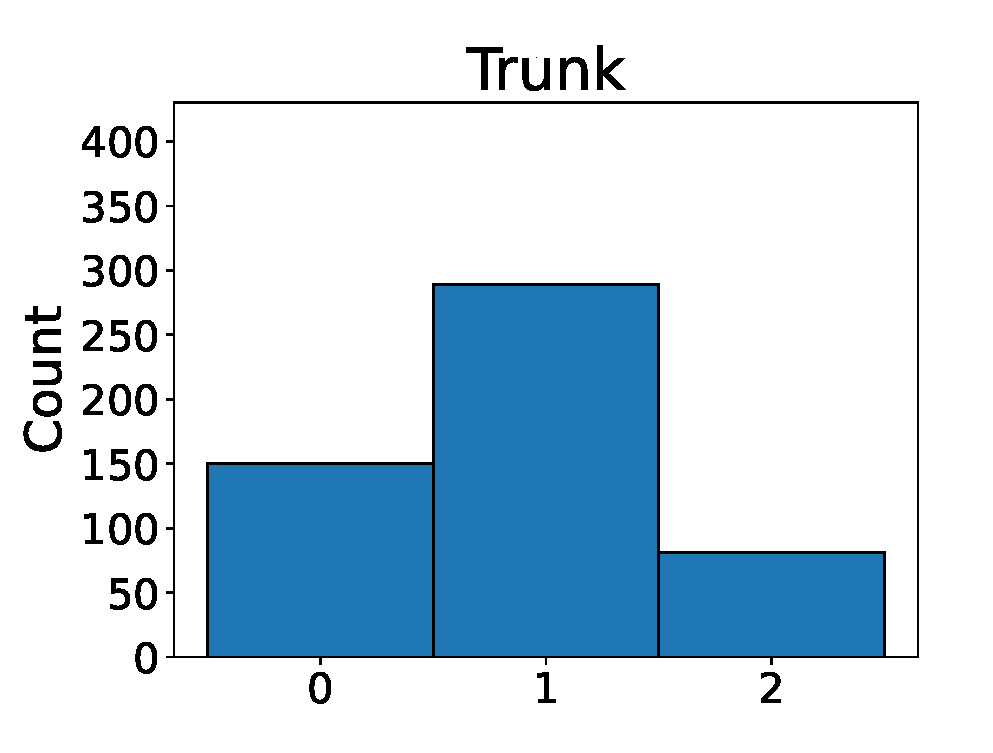
\includegraphics[width=\textwidth]{files/figs/met/trunk-label-hist.eps}
    \caption{}
    \label{fig:trunk-labels}
  \end{subfigure}
  \begin{subfigure}[t]{0.24\textwidth}
    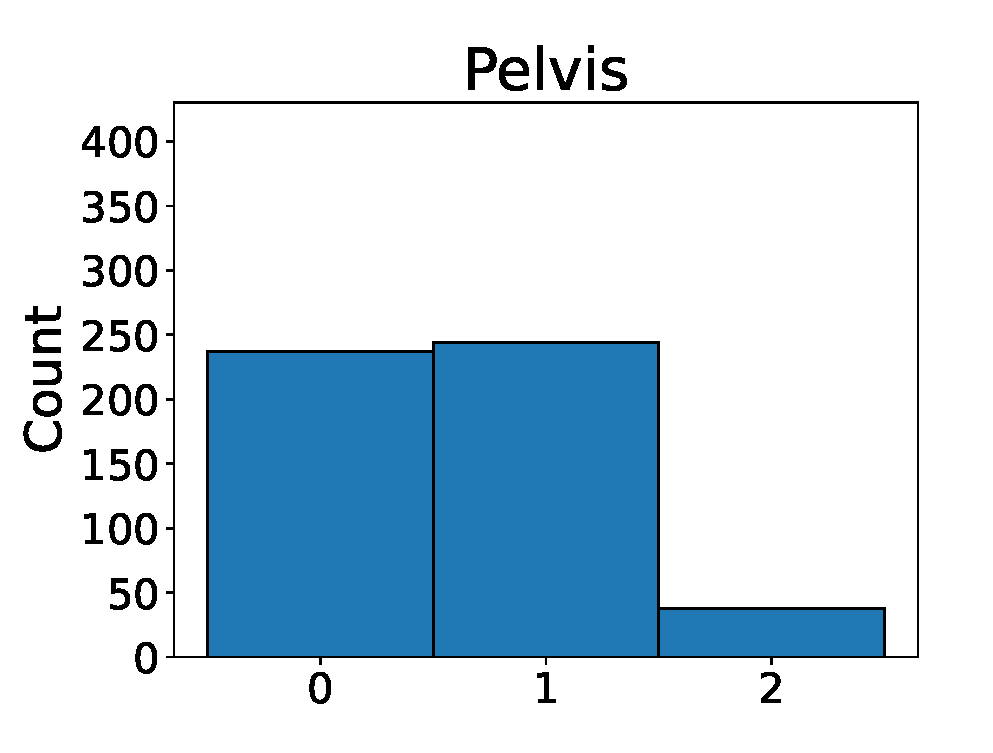
\includegraphics[width=\textwidth]{files/figs/met/pelvis-label-hist.eps}
    \caption{}
    \label{fig:pelvis-labels}
  \end{subfigure}
  \begin{subfigure}[t]{0.24\textwidth}
    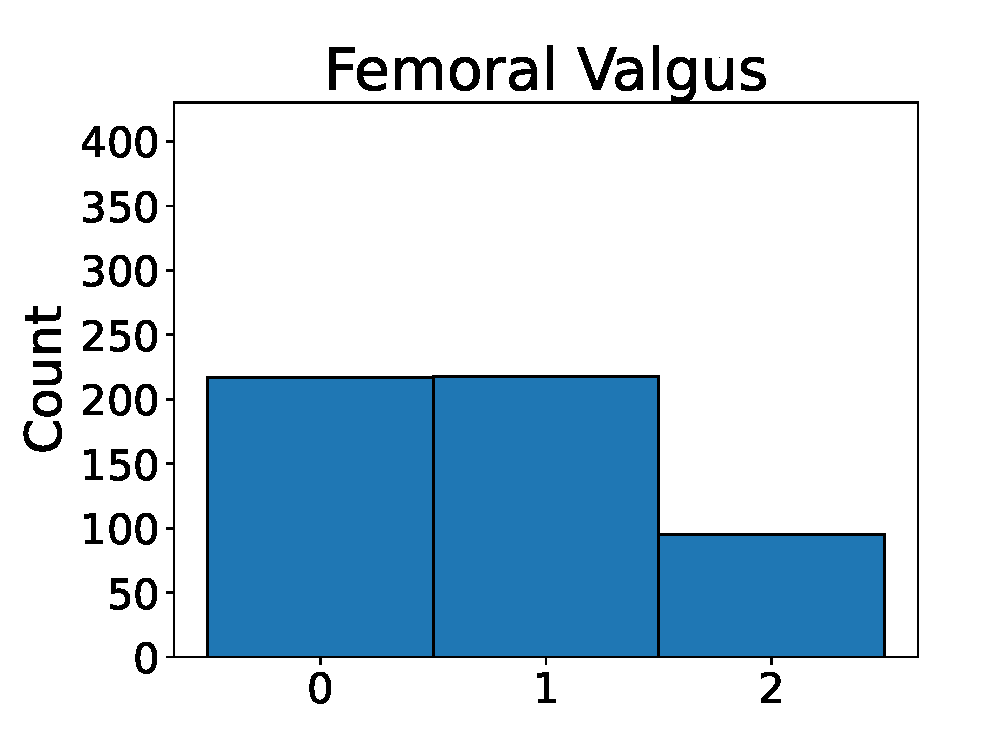
\includegraphics[width=\textwidth]{files/figs/met/femval-label-hist.eps}
    \caption{}
    \label{fig:femval-labels}
  \end{subfigure}
  \begin{subfigure}[t]{0.24\textwidth}
    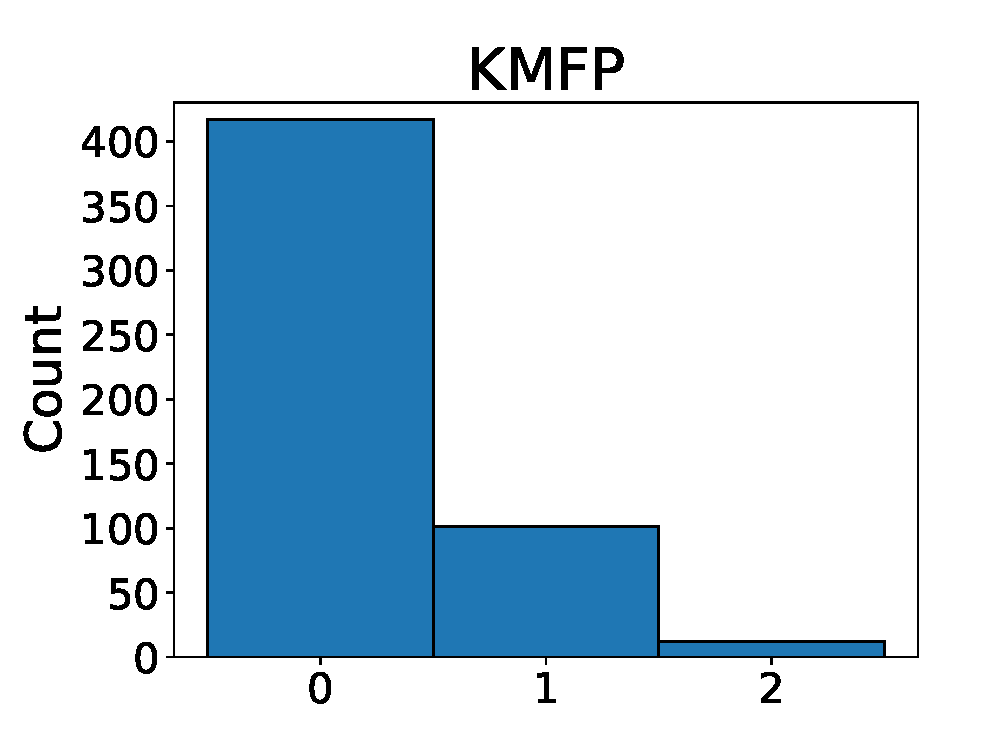
\includegraphics[width=\textwidth]{files/figs/met/kmfp-label-hist.eps}
    \caption{}
    \label{fig:kmfp-labels}
  \end{subfigure}

  \begin{subfigure}[t]{0.24\textwidth}
    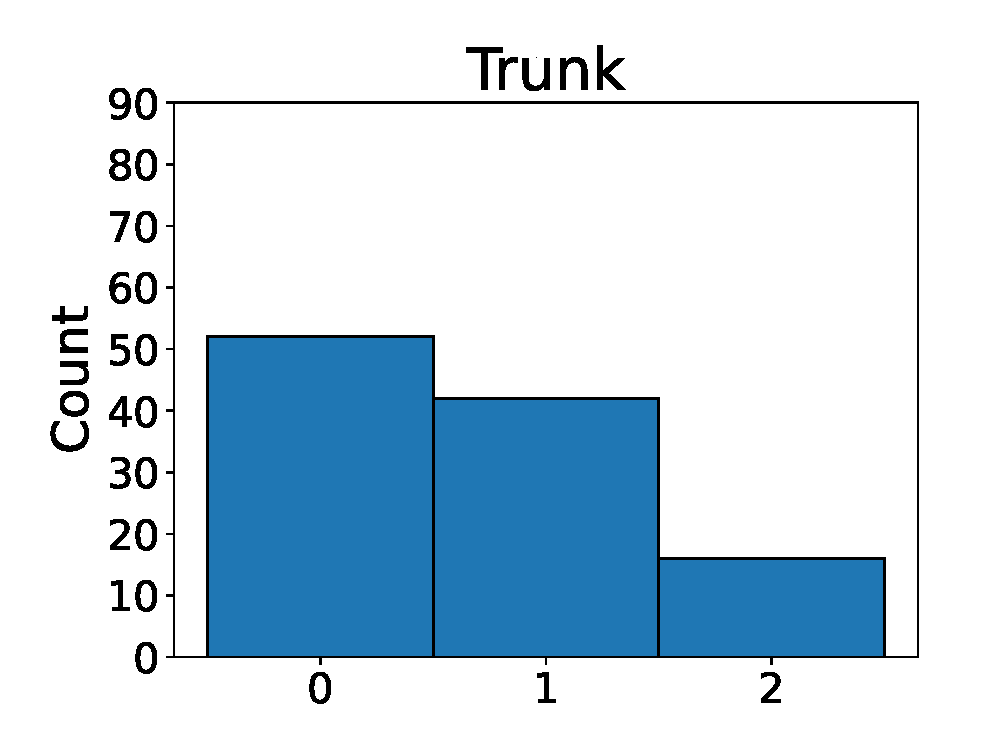
\includegraphics[width=\textwidth]{files/figs/met/trunk-test-labels.eps}
    \caption{}
    \label{fig:trunk-labels-test}
  \end{subfigure}
  \begin{subfigure}[t]{0.24\textwidth}
    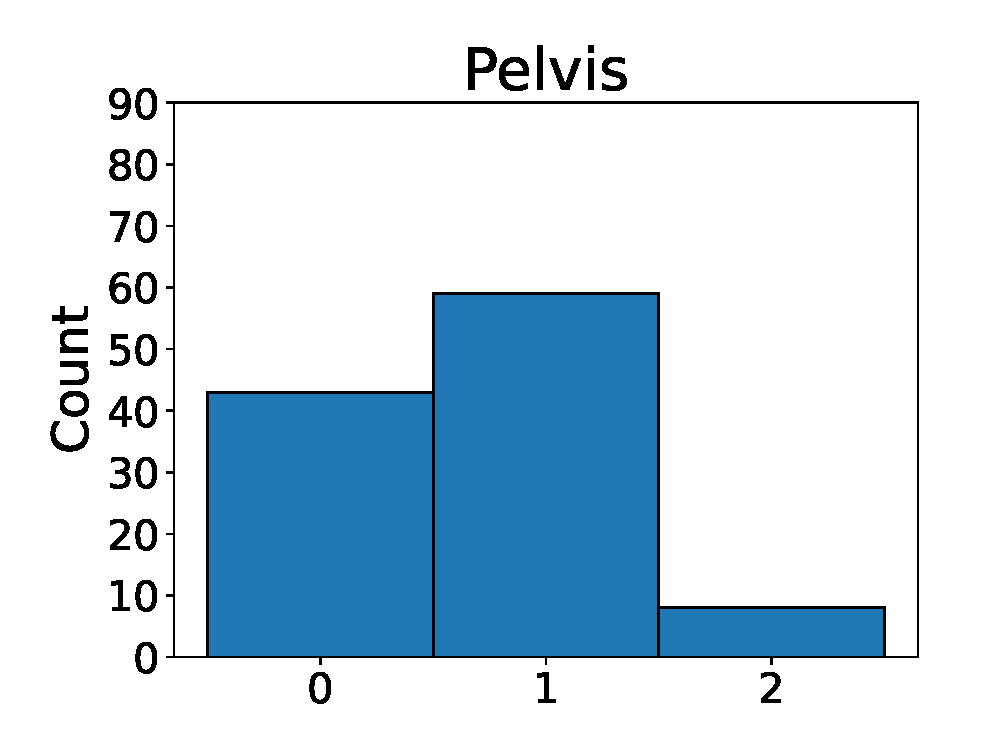
\includegraphics[width=\textwidth]{files/figs/met/pelvis-test-labels.eps}
    \caption{}
    \label{fig:pelvis-labels-test}
  \end{subfigure}
  \begin{subfigure}[t]{0.24\textwidth}
    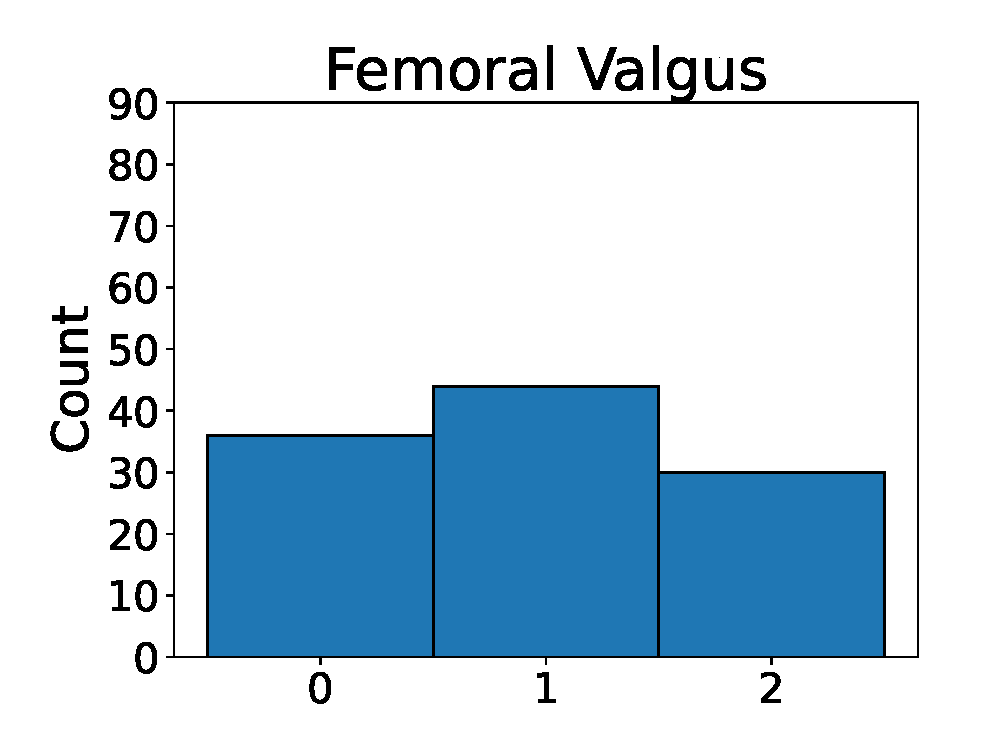
\includegraphics[width=\textwidth]{files/figs/met/femval-test-labels.eps}
    \caption{}
    \label{fig:femval-labels-test}
  \end{subfigure}
  \begin{subfigure}[t]{0.24\textwidth}
    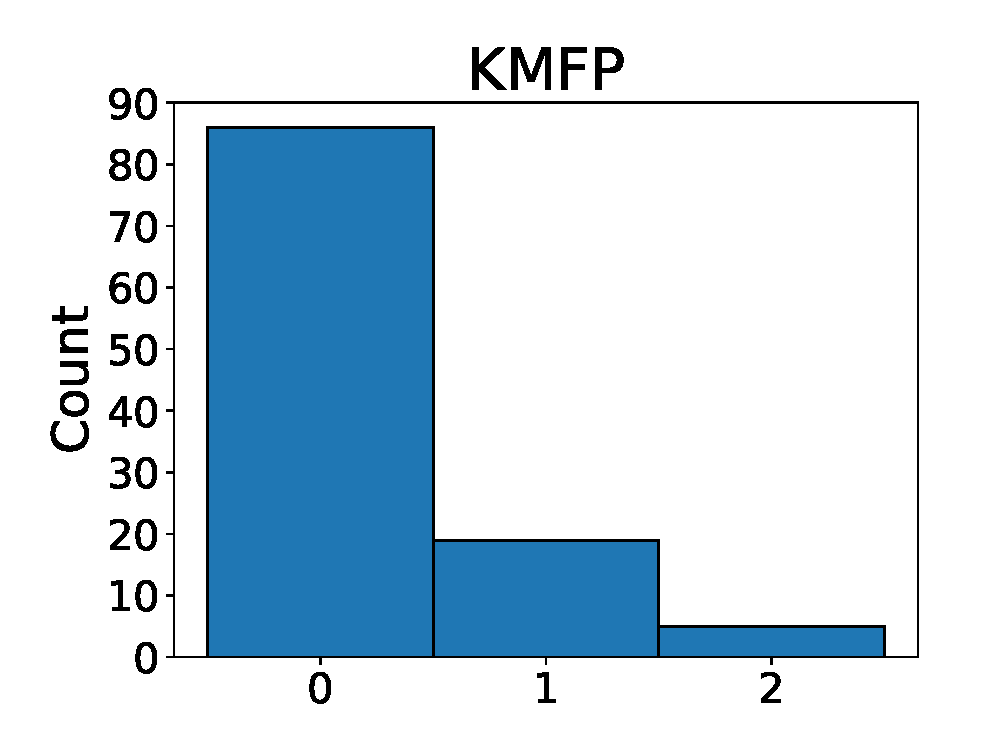
\includegraphics[width=\textwidth]{files/figs/met/kmfp-test-labels.eps}
    \caption{}
    \label{fig:kmfp-labels-test}
  \end{subfigure}

  \caption{Distributions of the labels for the available data. (a)-(d) shows distribution over all available data and (e)-(h) shows the distribution in the test set.}
  \label{fig:label-dist}
\end{figure}



\section{Body part localization} \label{sec:met-loc}
% \subsection{Preprocessing}
% ...
% rotation, flip etc
% \subsection{Pose estimation}
%The pose estimation can be seen as a feature extraction and dimensionality reduction.
The pose estimation is built around the open-source toolbox MMPose \cite{mmpose} from MMLab. Each frame is considered to be an independent image and is analyzed with a \gls{hrnet} model using the \gls{dark} extension trained on the \gls{coco}-wholebody dataset\footnote{The model used can be found here: \url{https://mmpose.readthedocs.io/en/latest/top_down_models.html}.}. Both the model and the dataset is described in Section \ref{sec:pose_estimation}. The extended wholebody dataset is used since it, along with the ankle positions, also estimates the positions of the toes and heels which contain valuable information. % \ref{sec:hrnet, sec:dark, sec:coco}.

To get comparable results some of the videos were rotated and flipped before inferring the keypoints. This was needed since the videos were recorded in different orientations and the actions were performed with different legs. The rotations were based on the orientation of the subject (position of head w.r.t. the feet) in the first frame to have it standing up in the $y$-direction. Videos where the squats were performed with the left leg were flipped around the $y$-axis to be able to use the same model for the left and right leg in a more efficient manner.

A bounding box for the subject is found using a Faster R-CNN model trained on the \gls{coco} dataset\footnote{The model used can be found here: \url{https://github.com/open-mmlab/mmdetection/tree/master/configs/faster_rcnn}.}. The content of this bounding box is resized to match the input size of the \gls{hpe} model used, 384$\times$288 pixels in our case. Each video analyzed results in sequences of $x$- and $y$-coordinates for all the keypoints in the dataset used to train the model.

%The file names contained information about which. The rotations were performed based on the position of the head with respect to the feet in the first frame.
\section{Classification} \label{sec:met-class}

\subsection{Preprocessing and creation of dataset} \label{sec:met-class-preproc}
Before assessing the \glspl{poe} based on the body part positions, a number of preprocessing steps are conducted. Firstly the data is resampled as the videos are recorded with a number of different frame rates ranging from 25 to 60 Hz. The resampling is performed using linear interpolation to a new sample frequency of 25Hz. This data is then low pass filtered through a fourth order Butterworth filter with a cutoff frequency of 5Hz. %PLOT P[ ;VERF;RING F;R FILTER? ELLER P[ FILTRERAD DATA?

While the \gls{poe} assessment is performed on a per repetition basis, the body part coordinates are extracted on a per video or repetition sequence basis. Hence, the sequences corresponding to the entire video is split up in the individual repetitions. This splitting is presented in Algorithm \ref{alg:rep} and is based on finding the edges of the peaks in specific position data. For the \gls{sls} task, the $y$-coordinate of the right shoulder is used. The number of points extracted for each repetition depends on the width of the peak. The length of the observed repetitions varies from about 1 to 8 seconds. For practical reasons, such as handling of data and training performance\footnote{All data in one batch must have the same size. Hence, to be able to train with a batch size larger than 1, which usually improves training performance \cite{Goodfellow2016}, all data in the same batch needs to have the same dimensions.}, it is desirable to save the data as multidimensional arrays with the same dimensions. Two different ways of solving this problem is evaluated, namely i) padding the sequences and use maskings for the padded samples in the models, and ii) alternate the sample frequency to thereby achieve sequences of the same length.
%Some number of points around each peak is  This is done by finding peaks in the sequences corresponding to certain body part positions. Which body part is used for this sequence splitting depends on which movement is analyzed.

\begin{algorithm}
\SetAlgoLined
% \KwResult{Write here the result }
%  initialization\;
% peaks, right\_edges, left\_edges = \textbf{find\_peaks}(sequence)\;
right\_edges, left\_edges = \textbf{find\_edges}(sequence)\;
 \For{\textup{peak, right, current\_left, next\_left} in \textup{peaks, right\_edges, left\_edges}}{
 % \For{\textup{peak, right, current\_left, next\_left} in \textup{peaks, right\_edges, left\_edges}}{
  split\_index = \textbf{mean}(right, next\_left)\;
  start = \textbf{max}(current\_left - extra\_points, 0)\;
  end = \textbf{min}(right + extra\_points, split\_index)\;
  % start = \textbf{max}(peak - max\_length/2, 0)\;
  % end = \textbf{min}(peak + max\_length/2, split\_index)\;
  \textit{repetition} = \textbf{normalize\_length}(sequence[start:end])\;
  sequence = sequence[end:]\;
 }
 \caption{Extraction of repetitions from sequences}
 \label{alg:rep}
\end{algorithm}


Finally, the data is normalized. All coordinates are moved to put the mean position of the first five right hip-samples in the origin and are scaled to set the distance between the right shoulder and right hip to one, according to

\begin{align}
  \begin{split}
    (x,y)_i &= (x,y)_i - {\mean{(x,y)}}_{rh} \\
    (x,y)_i &= \frac{(x,y)_i}{\lVert \mean{(x,y)}_{rs} \rVert_2} \qquad , \forall i
  \end{split}
  \label{eq:met-normalization}
\end{align}
where $\mean{(x,y)}_i$ denotes the mean over first five samples for body part $i$, \textit{rh} the right hip, \textit{rs} the right shoulder, and \textit{i} the different bodyparts.

After these preprocessing steps, a dataset with inputs $\in \mathbb{R}^{N \times T \times F}$ and corresponding one-hot labels $\in \mathbb{Z}_3^N$ are created. The inputs consists of $N$ multivariate time series of length $T$ with $F$ channels. These channels are a subset of the extracted $x$- and $y$-coordinates as well as angles and differences between keypoints. Which features are used and how they are chosen are presented in Section \ref{sec:met-inputs}.

\subsection{Classifiers}
For the modeling, we used ensembles of different deep learning based model architectures. The reasoning behind this was based on the results of Fawaz et al. \cite{IsmailFawaz2019ensemble}, suggesting that the output a deep learning model trained on a limited amount of data will vary based on the initial parameter values. By averaging the result over several models this variance will be reduced. Another reason for using an ensemble is, as can be seen in e.g. \cite{Bagnall2015, Lines2016}, that the combined result of many specialized models can be better than that of one more general model. %In this work it for instance mean that we can train models with the confusion-entropy loss \eqref{eq:confusion-entropy} to achieve e.g. high precision for just one class in combination with models trained with the \gls{coral} loss \eqref{eq:coral-loss} performing fairly good over all classes.

All models used have been modified to handle the padded input data discussed in Section \ref{sec:met-class-preproc}. This is done by adding masking layers setting the padded samples to zero throughout the networks, as illustrated in Figure \ref{fig:x-inception}. This reduces the impact of the padded samples to something similar to the padding performed in convolutional layers to keep the size of the feature map intact. The same mask indicates which time steps should be ignored in the \gls{gap} layer.

The models eventually used were InceptionTime (Section \ref{sec:inception-time}) with different loss functions as well as an architecture designed by us, inspired by
\gls{xcm} (Section \ref{sec:XCM}) and InceptionTime. We call this model X-InceptionTime and it is presented below.

\subsubsection{X-InceptionTime} \label{sec:xinception}
The idea with this model was to combine the explainability of XCM with the inception module from InceptionTime. This was done by separating the inputs and having individual inception modules for each input channel as can be seen in Figure \ref{fig:x-inception}. After the final module (the depth can be seen as a hyperparamtere and needs to be tuned) a bottleneck of size one is applied reducing the dimensionality of each input channel back to $T$$\times$1. The features for the individual inputs are concatenated resulting in a feature map of size $T$$\times$$F$ where each input feature is only affected by that input. This makes it possible to use \gls{grad-cam} to get a measure of the importance of each time step for each input.

\begin{figure}
  \centering
  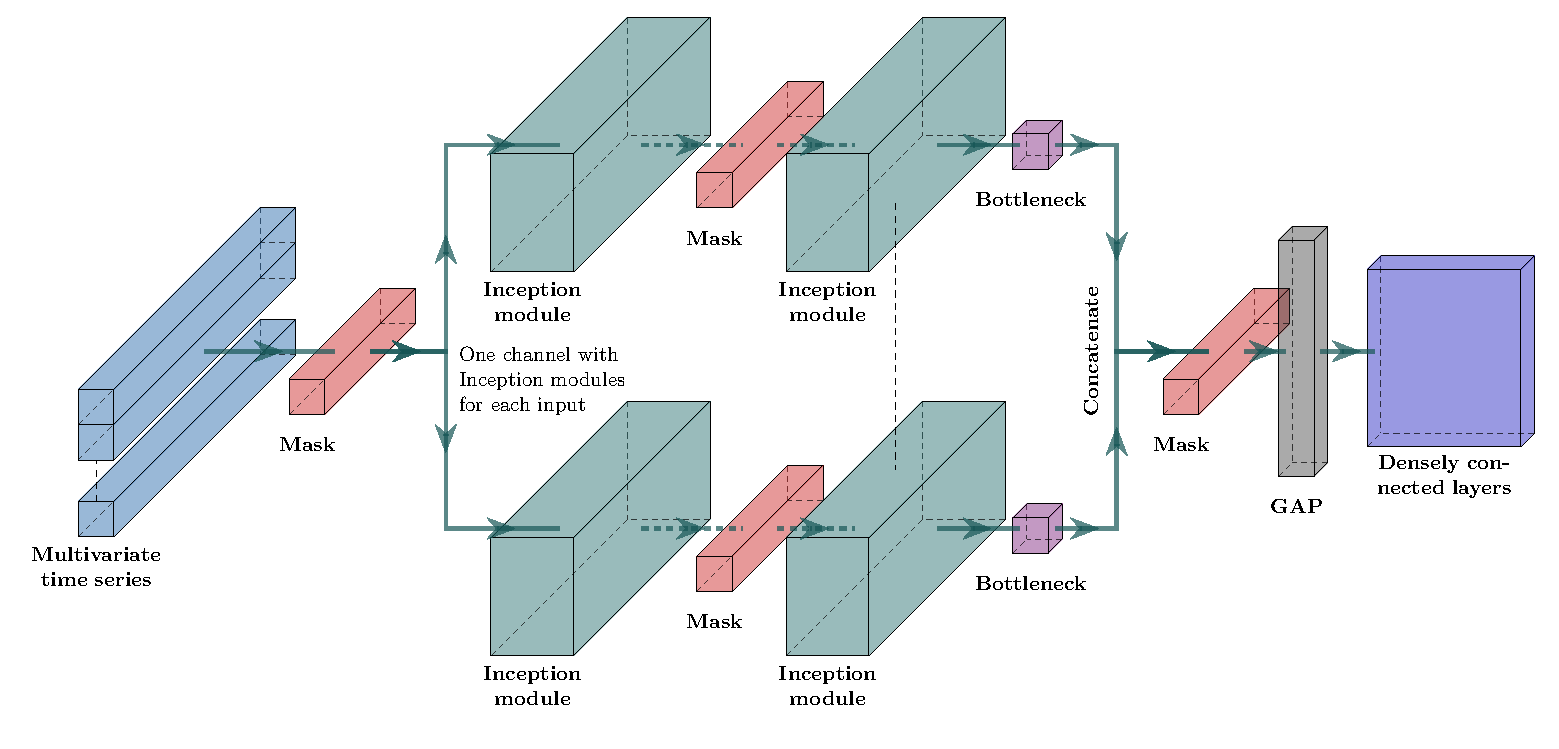
\includegraphics[width=\textwidth]{files/figs/met/x-inception-w-masks.pdf}
  \caption{The X-InceptionTime architecture developed in this work.}
  \label{fig:x-inception}
\end{figure}

The \gls{grad-cam} method is slightly modified and simplified for this model compared to what is presented in Section \ref{sec:grad-cam}, mainly due to the one dimensional data. Consider the final feature map $A$ consisting of the concatenated feature maps from the separate input channels. As mentioned above $A \in \mathbb{R}^{T \times F}$ and the aim is to find importance values for each time step in each input. With the same notations as in \eqref{eq:grad-cam}, i.e. $A_i^k$ corresponds to the activation of input $k$ at time step $i$, the \gls{grad-cam}, $M_c^k$, for class $c$ and input $k$ can be calculated as follows

\begin{align}
    \begin{split}
        w_k^c &= \frac{1}{T}\sum_{i=1}^T \frac{\partial y_c}{\partial A_i^k} \\
        M_c^k &= w_k^c A^k.
    \end{split}
    \label{eq:grad-cam-x}
\end{align}

 Compared to \eqref{eq:grad-cam} the $ReLU$ activation has been removed. This means that the importance values also contain information about which features suggesting this sample belongs to another class than $c$.

 Along with the effect of the time steps it is also possible, thanks to the \gls{gap} layer, to get a measure of the importance of each input. The importance value, $\alpha_k^c$, for input $k$ describes how much effect this input has on the classification decision. It is given by applying the \gls{grad-cam} method to the output of the \gls{gap} layer, $B$. From the feature map, $A$, this importance weight is calculated according to

 \begin{align}
   \begin{split}
      B^k &= \frac{1}{T}\sum_{i=1}^T A_i^k \\
      w_k^c &= \frac{\partial y_c}{\partial B^k} \\
      \alpha_k^c &= w_k^c B^k.
      \label{eq:input-importance}
   \end{split}
 \end{align}


\subsubsection{Ensembles} \label{sec:met-ensembles}
The ensembles used consists of multiple models whose outputs are linearly combined to form the ensemble output. As discussed above, this allows the ensemble to benefit from models optimized to perform well according to different metrics. In Section \ref{sec:met-training}, we will present how $k$-fold cross-validation was used for training and validation. This was also used for design of the ensembles.

The idea with the ensemble was to combine models performing across all classes with models with high precision for the individual classes. The models with good overall performance was in general using the \gls{coral} activation and loss. The other models were trained with the confusion entropy loss with a target confusion matrix, from which the $u_{ij}$ in \eqref{eq:confusion-entropy} comes, aiming at achieving high precision for one class and ignoring the other predictions. Examples of matrices used to find high precision models are

\noindent\begin{subequations}
\begin{minipage}{.33\textwidth}
  \begin{align}
  \label{eq:target-0}
  \begin{bmatrix}
    0.6 & 0.05 & 0.05 \\
    0 & 1 & 1\\
    0 & 1 & 1
  \end{bmatrix}
\end{align}
\end{minipage}%
\begin{minipage}{.33\textwidth}
  \begin{align}
  \label{eq:target-1}
  \begin{bmatrix}
    1 & 0 & 0 \\
    0.3 & 0.5 & 0.3\\
    0 & 0 & 1
  \end{bmatrix}
\end{align}
\end{minipage}%
\begin{minipage}{.33\textwidth}
  \begin{align}
  \label{eq:target-2}
  \begin{bmatrix}
    1 & 1 & 0 \\
    1 & 1 & 0 \\
    0.1 & 0.1 & 0.4
  \end{bmatrix}.
\end{align}
\end{minipage}
\label{eq:confusion-target}
\end{subequations}

A higher value can be seen as a reward for predictions turning up at that position in the confusion matrix and clearly the sum of the columns are not equal, meaning that the models will be biased towards certain predictions. Eq. \eqref{eq:target-0} is used for class 0 and the ones in the lower right corner in this example means that correct prediction of a 1 will give the same reward as incorrectly predicting it as a 2.
The idea behind the lower reward for correct prediction of 0 together with the small rewards for predicting it as a 1 or 2 is to classify uncertain examples as 1s or 2s. The idea for class 2, in \eqref{eq:target-2} is the same, but opposite. As the underlying scoring scale is ordinal, the same approach was not suitable for class 1. Instead a target matrix like \eqref{eq:target-1} was used. An alternative way of achieving high precision models was to tune the weight parameters $\lambda$ in the \gls{coral} loss, \eqref{eq:coral-loss}, to emphasize one of the rank predictions over the other.
Due to the significant class imbalance for the \gls{kmfp} \gls{poe} the goal for class 1 and 2 was not to achieve high precision. Instead models slightly biased towards these classes were used. This was achieved by using confusion entropy losses with target matrices shown in Appendix \ref{app:models-kmfp}.

For the ensemble output the outputs of the individual models were combined as a weighted sum, initially according to
\begin{subequations}
\begin{align}
      \mybar[0.7][1pt]{y}^{(c)} &= \sum_{i=1}^E w_i^{(c)} \widehat{y}_i^{(c)}, \\
      1 &= \sum_{i=1}^E w_i^{(c)}, \quad \forall c, \label{eq:weight-sum}
\end{align}
\end{subequations}
where $E$ denotes the number of ensembles, $\mybar[0.7][1pt]{y}$ the ensemble output, and $\widehat{y}_i$ the output of the $i$-th model.
% \begin{conditions}
%   E                   & = & number of ensembles \\
%   \mybar[0.7][1pt]{y} & = & ensemble output \\
%   \widehat{y}_i       & = & output if the $i$-th model.
% \end{conditions}

The models used were determined based on the performance during the cross-validation and the weights were chosen uniformly for all models except the high precision ones. For these the weights instead were set to zero for the classes it was not trained for. By studying the predicted output probabilities for the validation data it could be seen that they in some cases were slightly biased away from class 1. The histogram of the predicted class 1 probabilities for the Femoral Valgus data is shown in Figure \ref{fig:prob-1}. The main reason for this bias is the \gls{coral} classifier which tends to result in slightly lower predictions for intermediary classes. To prevent this from resulting in skewed combined scores (see Section \ref{sec:met-combined}) the weights for this class were increased slightly, resulting in \eqref{eq:weight-sum} summing to something greater than one for class 1. The final ensemble weights can be seen in Appendix~\ref{app:models}. The weights for all models in the ensemble were multiplied with the same factor, resulting in the adjusted histogram in Figure \ref{fig:prob-adjusted}. This adjustment shifts all probabilities, but will have a greater effect for predictions with already high probability.

\begin{figure}[h]
  \centering
  \begin{subfigure}[t]{0.45\textwidth}
  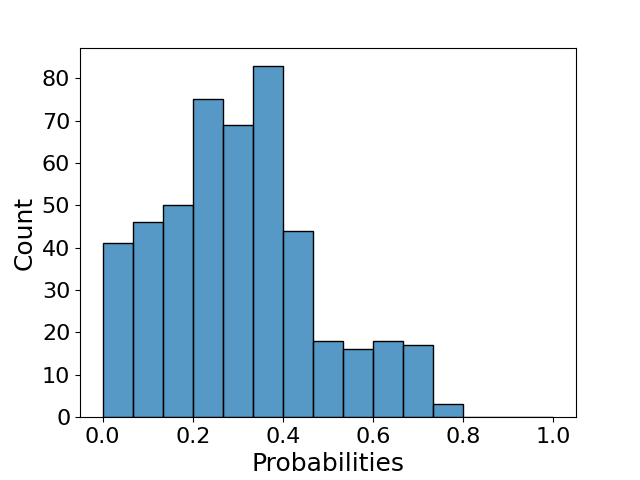
\includegraphics[width=\textwidth]{files/figs/met/probs-1.png}
  \caption{}
  \label{fig:prob-1}
\end{subfigure}
~
\begin{subfigure}[t]{0.45\textwidth}
  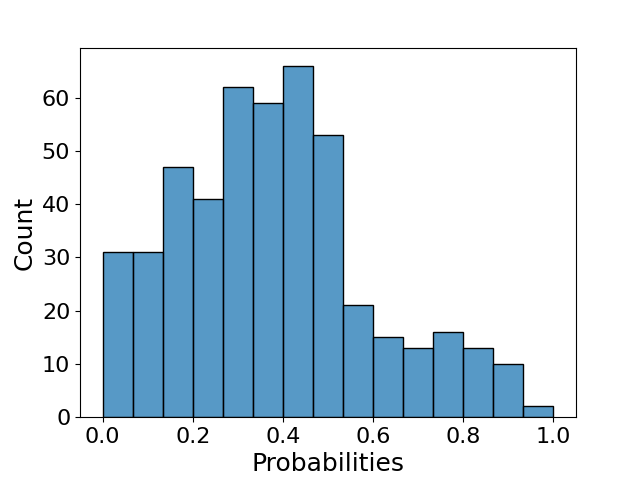
\includegraphics[width=\textwidth]{files/figs/met/probs-1-adjusted.png}
  \caption{}
  \label{fig:prob-adjusted}
\end{subfigure}
  \caption{Output probabilities for class 1 (Femoral Valgus) from the unadjusted (a) and adjusted (b) ensemble suggesting some bias away from this label.}
  \label{fig:bias-1}
\end{figure}

The ensembles used are presented in Table \ref{tab:ensemble-models}. The suffixes -coral and -conf-X indicates \gls{coral} classifiers and models trained with the confusion entropy loss, respectively. The X tells which was the high precision class. This is also used to indicate \gls{coral} models trained to achieve high precision. The depth, filter length, and number of filters for all X-InceptionTime models were 1, 31, and 32. The corresponding parameters for the InceptionTime models were 2, 31, and 128. All models use Leaky-\gls{relu} activations throughout the network. More detailed model descriptions can be found in Appendix \ref{app:models} along with its training and ensemble weights.

\begin{table}
 \centering
 \caption{Models forming the ensembles. * indicates data length normalized to 100 samples. No star means that original sample frequency (25Hz) was kept and the input data was padded to the same length. If neither coral nor conf is stated cross entropy loss is used. IT shows InceptionTime modules were used. The identifier TX, PX, FX, KX is used in Appendix \ref{app:models} where more information, such as ensemble and training weights, can be found.}
 \label{tab:ensemble-models}
 % \footnotesize
 % {\renewcommand{\arraystretch}{1.2}
 % {\tabulinesep=0.8mm
 \small
 \begin{tabu}[t]{l:l:l:l}
   \textbf{Trunk} & \textbf{Pelvis} & \textbf{Femoral Valgus} & \textbf{\gls{kmfp}} \\
   \hline \hline
   T1, IT-coral*     & P1, IT-coral*      & F1, IT-coral*    & K1, IT \\
   T2, IT-coral      & P2, IT-coral       & F2, X-IT-coral*  & K2, X-IT \\
   T3, X-IT-conf-0*  & P3, IT-conf-0*     & F3, X-IT-conf-0* & K3, X-IT-conf-0 \\
   T4, IT-conf-1*    & P4, IT-conf-1      & F4, X-IT-conf-1  & K4, IT-conf-1* \\
   T5, X-IT-coral-2* & P5, X-IT-coral-2*  & F5, X-IT-conf-2* & K5, X-IT-conf-2
 \end{tabu}
\end{table}

% The models we used in the ensembles can be divided into three categories, i) models with good overall performance, ii) models with high precision for a specific class, and iii) models with high recall for a specific class. We found regular cross entropy and \gls{coral} models be suitable for the first category. This category forms the base of the ensemble and also works as a baseline to compare against. Unless the ensemble performs better than these individual models it does not serve any purpose. The second category, models with high precision,


% coral osv. custom losses osv?

\subsection{Input selection} \label{sec:met-inputs}
To select which inputs to use when classifying the different \glspl{poe} the importance weight introduced in \eqref{eq:input-importance} was used. This was done by iteratively training models and evaluating

\begin{equation}
    W_k = \text{mean\_folds}\Big( \text{normalize}(\sum_{i=1}^N |w_{ik}^{c_i}|) \Big),
    \label{eq:feat-select}
\end{equation}
where $\text{mean\_folds}(z)$ denotes the average of $z$ over all folds, $\text{normalize}(z) = \frac{z}{\lVert z \rVert_2}$, and $c_i = \text{argmax}(\hat{y}_i)$, i.e., the predicted class.

For each set of inputs evaluated the features corresponding to the lowest $W_k$ were removed until the performance of the model dropped significantly. This method has its drawback, the most notable being that only input features suitable for this architecture will be found. This model does not consider interaction between different features directly as the inputs are kept separate throughout the network, hence features important through such interactions might not be deemed important. This was somewhat circumvented by validating the reduced input features on other model architectures as well, allowing this methodical way of finding suitable inputs. The inputs used for the different \glspl{poe} are presented in Table \ref{tab:model-inputs}.



\begin{table}
  \caption{Inputs to the models classifying the different POEs. If the task was performed with the left leg the video has been mirrored, as described in Section \ref{sec:met-loc}.}
  \label{tab:model-inputs}
    \begin{center}
        \tabulinesep=0.8mm
        \begin{minipage}[t]{0.25\textwidth}
          \begin{tabu}[t]{l}
            \textbf{Trunk} \\ \hline \hline
            Left shoulder - $x$\\
            Right shoulder - $x$\\
            Right shoulder - $y$\\
            Left hip - $x$\\
            Left hip - $y$\\
            Right hip - $x$\\
            \multicolumn{1}{l}{\begin{tabular}[l]{@{}l@{}}Difference: right\\ hip and knee - $x$\end{tabular}}
          \end{tabu}
        \end{minipage}%
        \begin{minipage}[t]{0.25\textwidth}
          \begin{tabu}[t]{l}
            \textbf{Pelvis} \\ \hline \hline
            Right shoulder - $x$\\
            Right shoulder - $y$\\
            Right hip - $x$\\
            Right hip - $y$\\
            Left hip - $y$\\
            \multicolumn{1}{l}{\begin{tabular}[l]{@{}l@{}}Difference: right\\ hip and knee - $x$\end{tabular}}\\
            \multicolumn{1}{l}{\begin{tabular}[l]{@{}l@{}}Difference: right\\ knee and toes - $x$\end{tabular}}
          \end{tabu}
        \end{minipage}%
        \begin{minipage}[t]{0.25\textwidth}
          \begin{tabu}[t]{l}
            \textbf{Femoral Valgus} \\ \hline \hline
            Right shoulder - $x$\\
            Right hip - $x$\\
            Right knee - $y$\\
            \multicolumn{1}{l}{\begin{tabular}[l]{@{}l@{}}Angle: right\\ knee and ankle\end{tabular}}
          \end{tabu}
        \end{minipage}%
        \begin{minipage}[t]{0.25\textwidth}
          \begin{tabu}[t]{l}
            \textbf{\gls{kmfp}} \\ \hline \hline
            Left shoulder - $y$\\
            Right hip - $y$\\
            \multicolumn{1}{l}{\begin{tabular}[l]{@{}l@{}}Angle: right\\ ankle and toes\end{tabular}}\\
            \multicolumn{1}{l}{\begin{tabular}[l]{@{}l@{}}Difference: right\\ hip and knee - $x$\end{tabular}} \\
            \multicolumn{1}{l}{\begin{tabular}[l]{@{}l@{}}Difference: right\\ knee and ankle - $x$\end{tabular}} \\
            % \multicolumn{1}{l}{\begin{tabular}[l]{@{}l@{}}Difference: right\\ knee and ankle - $x$\end{tabular}}
          \end{tabu}
        \end{minipage}%
    \end{center}
\end{table}

\subsection{Training} \label{sec:met-training}
We used 10-fold cross-validation on the training set for the development of the models and ensembles. The amount of data used for training ranges from 74-77 sequences of repetitions and 369-380 repetitions for the different folds and \glspl{poe}. Like the test set, the folds were created such that no repetitions from the same subject were in both the test and validation set. For all models a batch size of 32, a learning rate of $5 \times 10^{-3}$, the Adam optimizer, and early stopping was used. The learning rate was also reduced by a factor of 0.85 every 50th epoch. The training was performed on Nvidia Tesla T4 and V100 \glspl{gpu}.

% \subsection{Choice of input features}

\subsection{Combined score} \label{sec:met-combined}
The eventual score in the method proposed by Nae et al. \cite{Nae2020b} is the combined assessments of all the repetitions. This score is formed as the median of the repetition scores. We propose to do this by averaging the ensemble outputs instead and chose the class with highest average probability over all repetitions. This means that a repetition classified with some uncertainty will affect the combined score less than a certain one. By evaluating the distributions for the ensemble outputs (Appendix \ref{app:val-hists}) it is also possible to introduce thresholds for both the combined score and the repetition score. For the repetition predictions the probability was set to 0 if the prediction was below 0.2. The validation data also suggests that the combined probability should work as an indicator of the certainty of the prediction. It could also be used to introduce a threshold ignoring predictions below a certain confidence. Studying the histograms, based on the validation sets in the cross-validation, in Appendix~\ref{app:val-hists}, a threshold of 0.4 seems to give a reasonable trade-of between ignored correct and incorrect samples.


\subsection{Baseline method} \label{sec:met-baseline}
The models presented above are compared to baseline methods using a large number of features combined with support vector machines and Fisher's linear discriminants. The features are extracted using the default options of tsfresh \cite{tsfresh}, i.e., no tuning of parameters or choice of features based on this specific problem has been performed. Examples of features used are number of peaks, mean values, derivatives of different orders, and variances.
